% Time-stamp: <2022-11-08 07:39:29 A13258Q>
% Amine Raboun 2023, https://amineraboun.github.io/
% Romain Lafarguette 2023, https://romainlafarguette.github.io/

%% ---------------------------------------------------------------------------
%% Preamble: Packages and Setup
%% ---------------------------------------------------------------------------
% Class 
\documentclass{beamer}

% Theme
\usetheme{Boadilla}
\usecolortheme{dolphin}
%\setbeamertemplate{headline}{} % Remove the top navigation bar

% Font and encoding
\usepackage[utf8]{inputenc} % Input font
\usepackage[T1]{fontenc} % Output font
\usepackage{lmodern} % Standard LateX font
\usefonttheme{serif} % Standard LateX font

% Maths 
\usepackage{amsfonts, amsmath, mathabx, bm, bbm} % Maths Fonts

% Graphics
\usepackage{graphicx} % Insert graphics
\usepackage{subfig} % Multiple figures in one graphic
\graphicspath{{/static/img}{/static/diagrams}}
\def\Z{\mathbb{Z}}
\def\R{\mathbb{R}}
\def\Esp{\mathbb{E}}
\def\Var{\mathbb{V}}
\def\Cov{\mathbb{C}ov}
\def\Corr{\mathbb{C}orr}
\def\Skew{\mathbb{S}}
\def\Kurt{\mathbb{K}}
\def\N{\mathcal{N}}
\def\F{\mathcal{F}}

% Layout
\usepackage{changepage}

% Colors
\usepackage{xcolor}
\definecolor{imfblue}{RGB}{0,76,151} % Official IMF color
\setbeamercolor{title}{fg=imfblue}
\setbeamercolor{frametitle}{fg=imfblue}
\setbeamercolor{structure}{fg=imfblue}

% Tables
\usepackage{booktabs,rotating,multirow} % Tabular rules and other macros
%\usepackage{pdflscape,afterpage} % Landscape mode and afterpage
%\usepackage{threeparttable} % Split long tables
\usepackage[font=scriptsize,labelfont=scriptsize,labelfont={color=imfblue}]{caption}

% Import files
\usepackage{import}

% Appendix slides
\usepackage{appendixnumberbeamer} % Manage page numbers for appendix slides

% References
\usepackage{hyperref}

% A few macros: environments
\newenvironment{wideitemize}{\itemize\addtolength{\itemsep}{10pt}}{\enditemize}
\newenvironment{wideenumerate}{\enumerate\addtolength{\itemsep}{10pt}}{\endenumerate}

\newenvironment{extrawideitemize}{\itemize\addtolength{\itemsep}{30pt}}{\enditemize}
\newenvironment{extrawideenumerate}{\enumerate\addtolength{\itemsep}{30pt}}{\endenumerate}

% Remove navigation symbols and other superfluous elements
\setbeamertemplate{navigation symbols}{}
\beamertemplatenavigationsymbolsempty

%\setbeamertemplate{note page}[plain]
\hypersetup{pdfpagemode=UseNone} % don't show bookmarks on initial view
\setbeameroption{hide notes}

% Institute font
\setbeamerfont{institute}{size=\footnotesize}
\DeclareMathSizes{10}{9}{7}{5}  

% Footnote without marker
\newcommand\blfootnote[1]{%
  \begingroup
  \renewcommand\thefootnote{}\footnote{#1}%
  \addtocounter{footnote}{-1}%
  \endgroup
}
%% ---------------------------------------------------------------------------
%% Title info
%% ---------------------------------------------------------------------------
\title[Time series Econometrics]{Time series Econometrics (Theory)}
\author[Lafarguette \& Raboun]{Romain Lafarguette, Ph.D. \and Amine Raboun, Ph.D.}
\institute[IMF STX]{Quants \& IMF External Experts\blfootnote{\scriptsize{\emph{This training material is the property of the IMF, any reuse requires IMF permission}}} \\
\begin{center}{\href{https://romainlafarguette.github.io/}{\textcolor{imfblue}{romainlafarguette.github.io/}} \hspace{0.3cm} \href{https://amineraboun.github.io/}{\textcolor{imfblue}{amineraboun.github.io/}}} \end{center} \vspace{-0.5cm}}

\date[STI, 17 April 2023]{Singapore Training Institute, 17 April 2023}

\titlegraphic{\vspace{-0.75cm}
    \begin{figure}
    \centering
    \subfloat{{
\includegraphics[width=2cm]{static/img/imf_logo}}}%
    \end{figure}}


% Slide between sections
\AtBeginSection[]
{
    \begin{frame}
        {Table of Contents}
        \tableofcontents[currentsection]
    \end{frame}
}
\AtBeginSubsection[]
{
    \begin{frame}
        {Table of Contents}
        \tableofcontents[currentsubsection]
    \end{frame}
}
%% ---------------------------------------------------------------------------
%% Title slide
%% ---------------------------------------------------------------------------
\begin{document}

\begin{frame}
\maketitle
\end{frame}
\begin{frame}
    \tableofcontents
\end{frame}

\section{Introduction}
\begin{frame}{Why Time series Modeling is different from other statistical models}

Why AR model is fundamentally different from an OLS?

Based on the model equation, AR is a special case of OLS where the explanatory variables are the lagged time series

$$AR(1): \quad y_t =\alpha + \beta \times y_{t-1} + \epsilon_t $$
$$OLS: \quad y_t =\alpha + \beta \times X_t + \epsilon_t $$

\medskip
\pause 
The hint to the answer is \textbf{Interpolation} vs \textbf{Extrapolation}
   
\end{frame}


\begin{frame}{OLS: Interpolation}
    \begin{columns}
        \begin{column}{.5\textwidth}
        \centering
        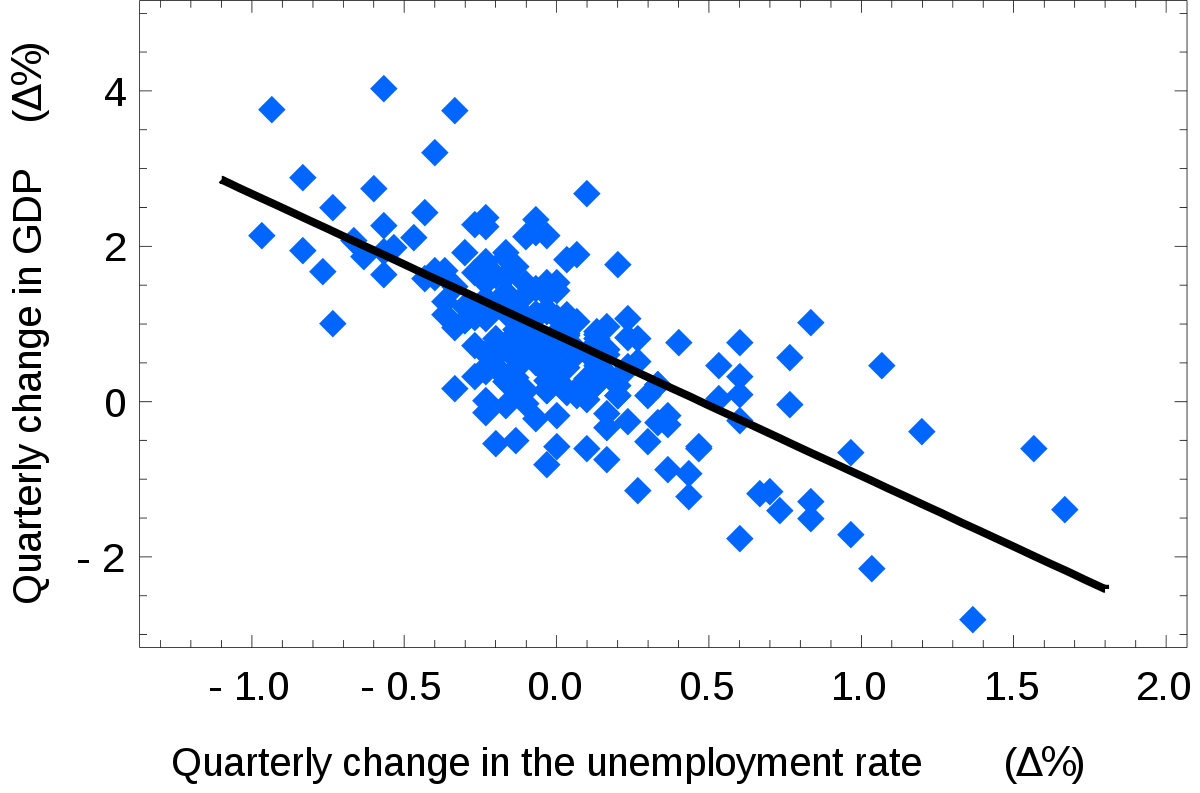
\includegraphics[width=\textwidth]{static/course_2_img/OLS_Interpolation.png}
        \end{column}
        
        \begin{column}{.5\textwidth}
        \begin{itemize}
            \item Both X and Y are observed at the same time. 
            \item For any potential value of X, we can compute a predicted value $\hat{Y}$ with a certain confidence
        \end{itemize}
        \end{column}
    \end{columns}

\end{frame}

\begin{frame}{AR: Extrapolation}
    \begin{columns}
        \begin{column}{.5\textwidth}
        \centering
        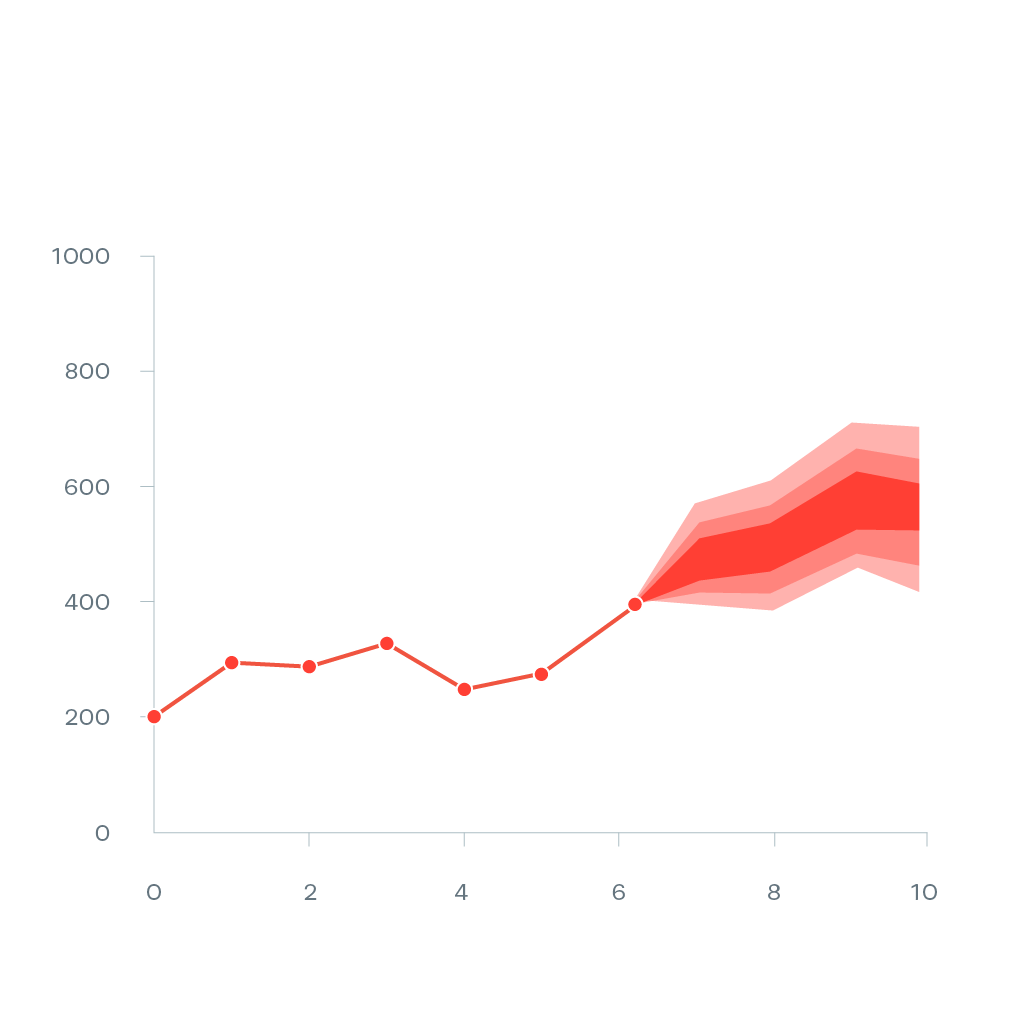
\includegraphics[width=\textwidth]{static/course_2_img/AR_Extrapolation.png}
        \end{column}
        
        \begin{column}{.5\textwidth}
        \begin{itemize}
            \item Structural time dependence, $\hat{Y}_{t+1}$ depend on $Y_{t}$
            \item Predicting $\hat{Y}_{t+h}$ requires predicting all $\hat{Y}_{t+i} \forall i \in [1,h-1]$
            \item Cumulative estimation error make the results unusable
        \end{itemize}        
        \end{column}
                 
    \end{columns}
Intuitively, the farther we move in the future,
    the higher the chance of exogenous external shock occurring (Risk of structured breaks, innovation, macroeconomic shocks, news...)
    => The lower the accuracy of the model        
\end{frame}
   
    
\section{Statistical Features and Properties of Financial Time series}

\begin{frame}
  {Stylized Properties}

  Fan and Yao (2015, the Elements of Financial Econometrics) identify 8 main "stylized facts"
  
  \begin{enumerate}
  \item Stationarity
  \item Absence of autocorrelations
  \item Heavy tails
  \item Asymmetry
  \item Volatility clustering
  \item Aggregational Gaussianity
  \item Long-range dependence
  \item Leverage effect
  \end{enumerate}
  
\end{frame}

\subsection{Stationarity}
\begin{frame}{Stationarity}

\begin{block}{Definition: Strong Stationarity }
    If ${y_t}$ is a stationary time series, then for any period $s$ in the future, the distribution $\{y_t, \dots, y_{t+s}\}$ doesn't depend on $t$
  \end{block}
 \medskip
 
 \begin{block}{Definition: Weak Stationarity (Second Order Stationarity)}
   A stochastic process $X_{t \in \mathbb{Z}}$ is weakly stationary if and only if:

   \begin{itemize}
   \item $\mathbb{E}(X^2_t) \ < \ \infty \ \quad \forall \ t \ \in \ \mathbb{Z}$
   \item $\mathbb{E}(X_t) = \mu \ \quad \forall \ t \ \in \ \mathbb{Z}$ doesn't depend on $t$
   \item $\text{Cov}(x_t, x_{t+h}) \ = \ \mathbb{E}[(x_{t+h} - m)(x_t - m)] \ = \ \gamma_h \quad \forall \ (t, h) \ \in \ \mathbb{Z}^2$ doesn't depend on $t$
   \end{itemize}
 \end{block}
 
\end{frame}

\begin{frame}{Intuitive Characterization}

A \textbf{stationary series} is:
  \begin{itemize}
  \item Roughly horizontal. The stochastic process oscillates around a constant level
      \begin{equation*}
\mathbb{E}(X_t) = \mu \forall t
\end{equation*}
  \item Constant variance. "\emph{covariance doesn't change when shifted in time}"
    \begin{equation*}
\mathbb{V}(X_t) = \mathbb{C}ov(X_t, X_{t}) = \gamma(0) \qquad \forall \ t \ \in \ \mathbb{Z}
  \end{equation*}
  \item No predictable patterns in the long term
  \end{itemize}
\end{frame}
  
\begin{frame}{Example}
\begin{exampleblock}{Fact N1:}
In general, prices are non-stationary but returns are stationary 
\end{exampleblock}  
\medskip
\centering
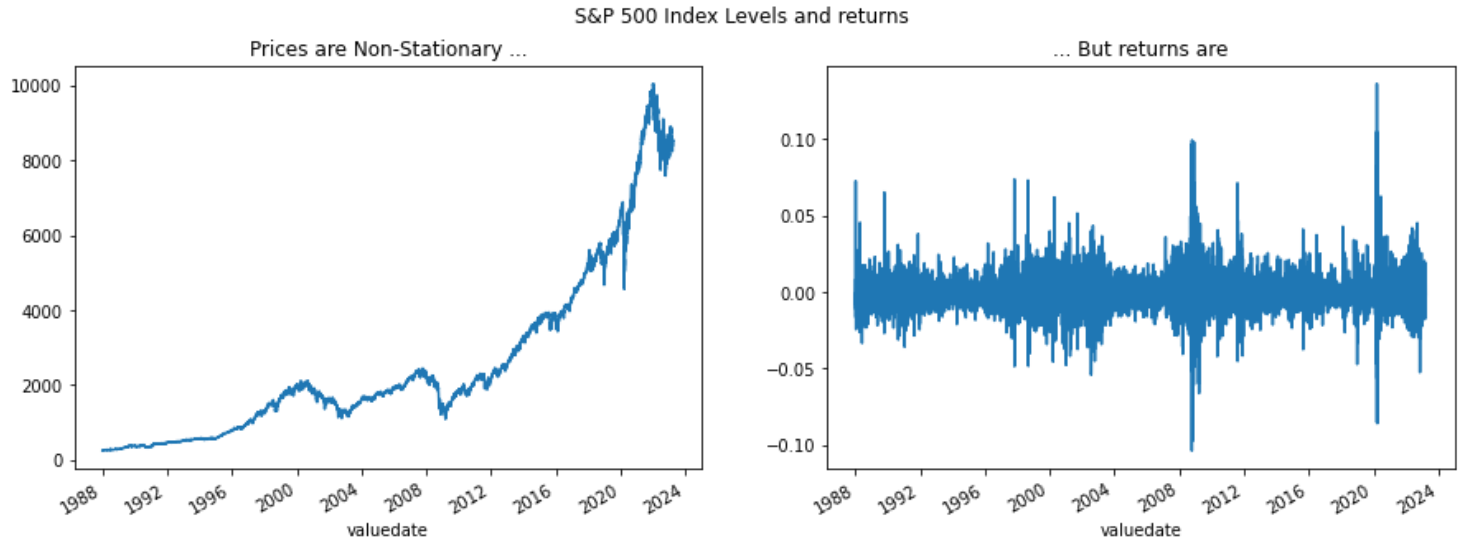
\includegraphics[width=\textwidth]{static/course_2_img/SP500_level_ret.PNG}           
\end{frame}

\begin{frame}{How do you identify non-stationary series?}
 Tips: It is easier to reject the stationarity of a time series rather than confirm it
 \medskip
\begin{enumerate}
    \item \textbf{Visually}: 
    \item \textbf{Global vs local}:
    \item \textbf{Compute the ACF}:    
    \item \textbf{Statistical tests}
\end{enumerate}
\end{frame}

\begin{frame}{Visually}
\begin{enumerate}
    \item \textbf{Visually}: the time plot gives information on the first moments throw time
\end{enumerate}
\medskip
\begin{columns}
    \begin{column}{.33\textwidth}
    \centering
    $\mu$ is not constant
    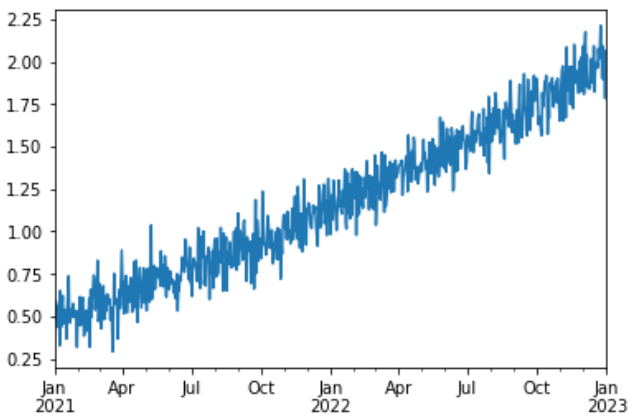
\includegraphics[width=\textwidth]{static/course_2_img/drift.PNG}           
    
    \end{column}
    
    \begin{column}{.33\textwidth}
    \centering
    $\sigma$ not constant
    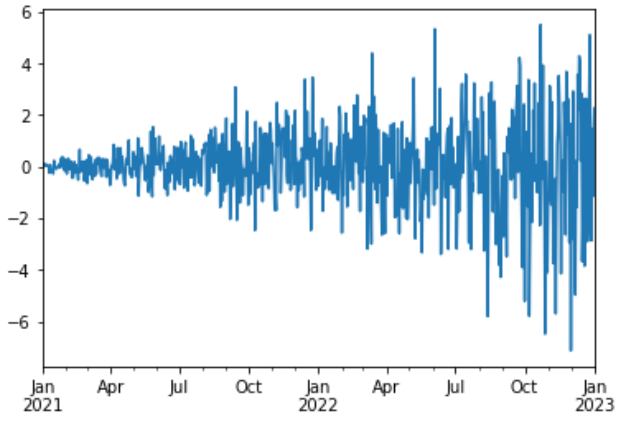
\includegraphics[width=\textwidth]{static/course_2_img/increasing_vol.PNG}        
    \end{column}
    
    \begin{column}{.33\textwidth}
    \centering
    Seasonal Pattern
    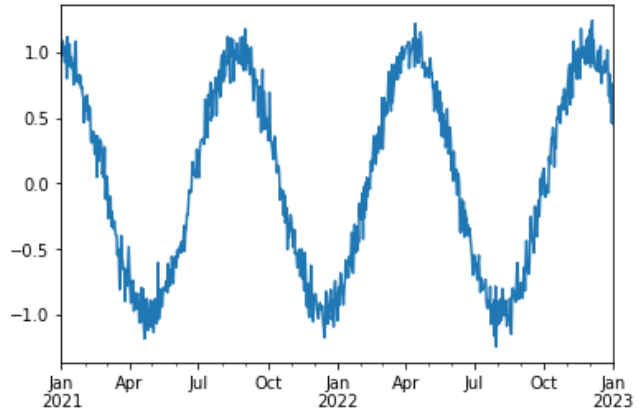
\includegraphics[width=\textwidth]{static/course_2_img/seasonal.PNG}     
    \end{column}
\end{columns}
\end{frame}

\begin{frame}{Global vs Local}
\begin{enumerate}
    \item[2.] \textbf{Global vs local}: compute the first moments locally and compare them with the global moments computed on the entire-time series
\end{enumerate}
Typical \textbf{structural breaks} can easily be identified by this technique 
\medskip

\begin{columns}
    \begin{column}{.7\textwidth}
        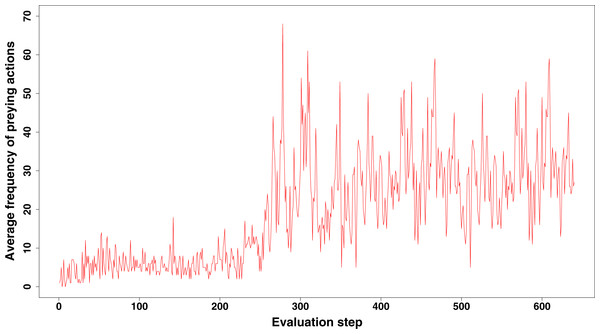
\includegraphics[width=\textwidth]{static/course_2_img/structural_break.jpg}  
    \end{column}
    \begin{column}{.3\textwidth}
        Double structural break:
\begin{itemize}
    \item Change in Mean 
    \item Increased Volatility
\end{itemize}
    \end{column}
\end{columns}
\end{frame}

\begin{frame}{ACF Analysis}
    \begin{enumerate}
    \item[3.] \textbf{Compute the ACF}:
    \begin{itemize}
        \item The ACF of stationary data drops to zero relatively quickly
        \item The ACF of non-stationary data decreases slowly
        \item For non-stationary data, the value of the first coefficient is often large and positive
    \end{itemize}
\end{enumerate}
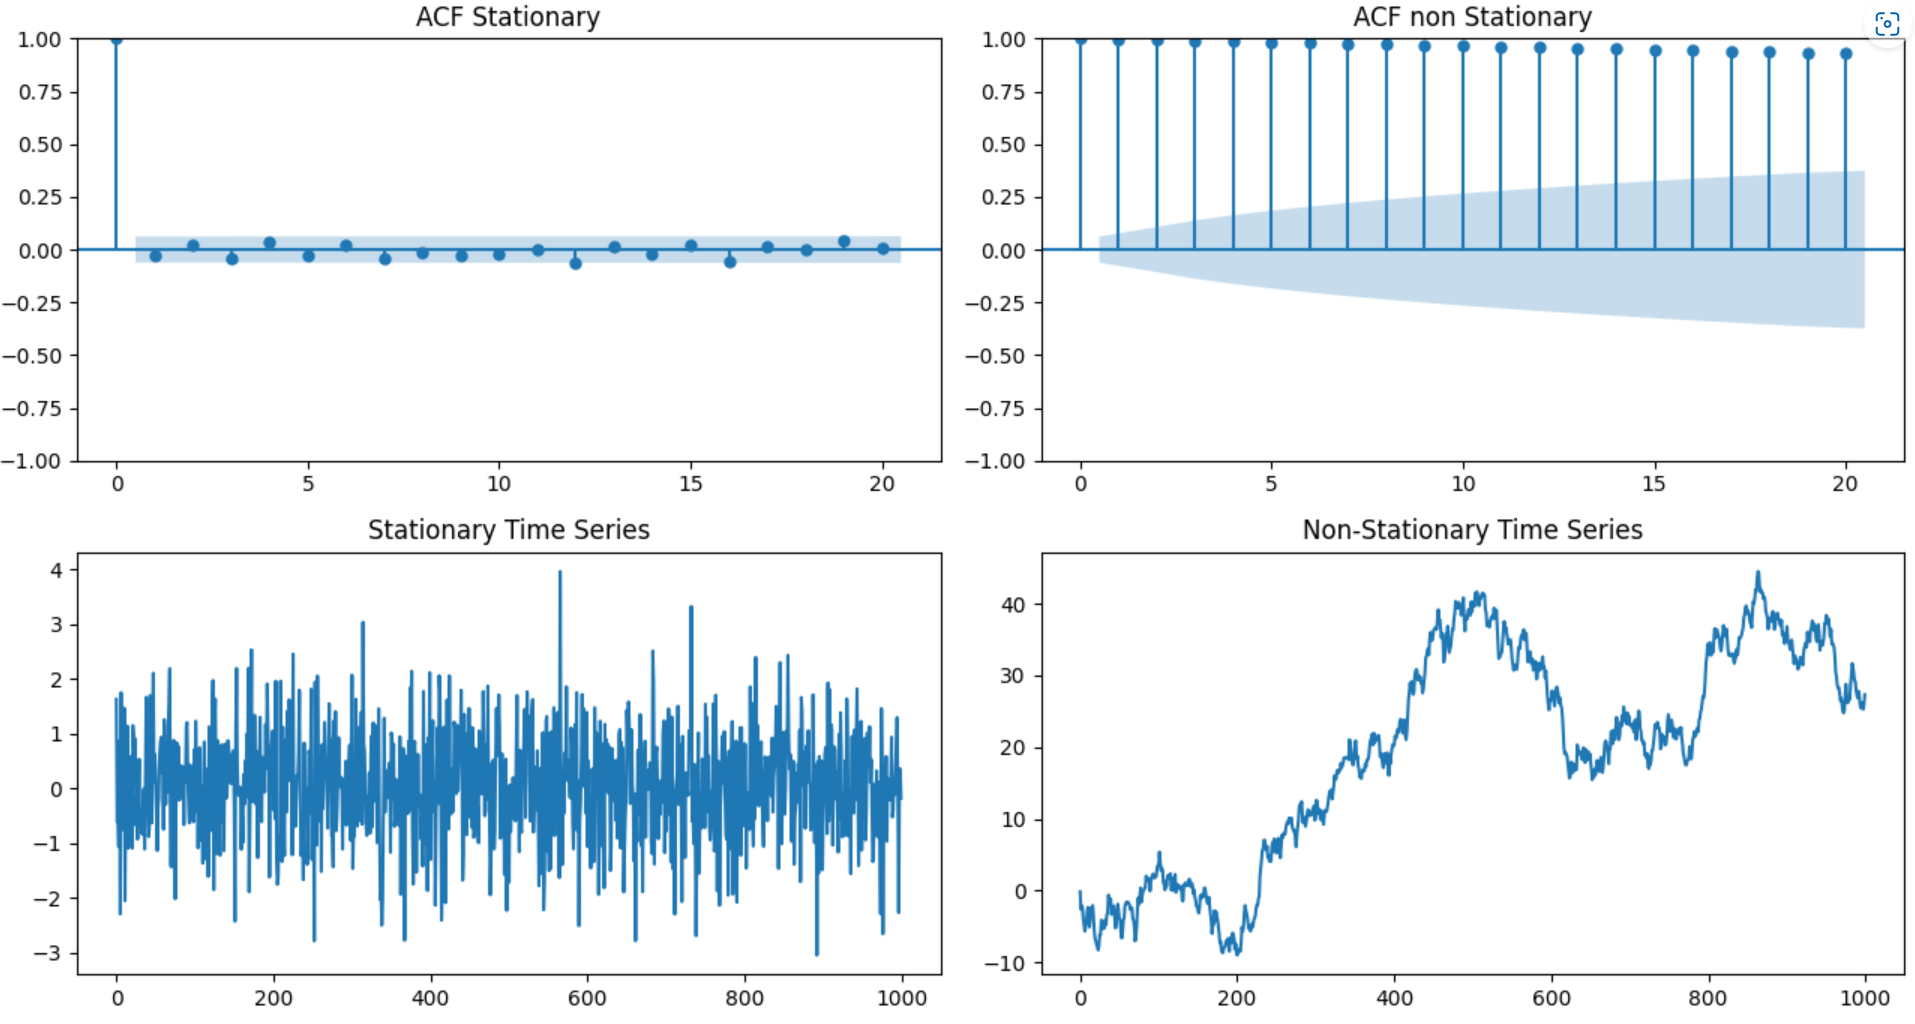
\includegraphics[width=\textwidth]{static/course_2_img/acf_stationary_nonstationary.PNG}  
\end{frame}

\begin{frame}{Unit Root Tests}
\begin{enumerate}
    \item[4.] Statistical tests for the presence of unit roots
\end{enumerate}
  
  \smallskip

  \begin{wideenumerate}
    \item \textbf{Augmented Dickey-Fuller test}: null hypothesis is that the data is \textbf{non-stationary} and non-seasonal
    \item KPSS (Kwiatkowski-Phillips-Schmidt Shin) test: the null hypothesis is that the data is \textbf{stationary} and non-seasonal
    \item Other tests are available for seasonal data
  \end{wideenumerate}
   
\end{frame}

\subsection{Absence of autocorrelations}
\begin{frame}{Absence of autocorrelations}
\begin{block}{Definition: Autocorrelation}
  The autocorrelation denoted $\rho(k)$ is the correlation between the values of the process at different times:

  \begin{equation*}
    \rho_k \ = \ \text{Corr}(X_t, X_{t-k}) \ = \ \frac{\mathbb{E}\left[ (X_t - \mu)(X_{t-k} - \mu)\right]}{\mathbb{V}(X_t)} = \frac{\gamma_k}{\sigma^2}
  \end{equation*}

with $\mu = \mathbb{E}[X_t]$, $\sigma^2 = \mathbb{V}(X_t), \ \forall \ t$ and $\gamma_k$ the autocovariance of order $k$  
\end{block}
\pause
  \begin{block}{Definition: Sample Autocorrelation}
    \begin{equation*} 
      \hat{\rho}_k = \text{corr}(X_t, X_{t-k}) = \frac{1}{(T-k)\hat{\sigma^2}} \sum_{t=k+1}^{R}(X_t - \hat{\mu})(X_{t-k} - \hat{\mu})
    \end{equation*}
where $\hat{\sigma^2}$ and $\hat{\mu}$ are consistent estimators of the mean $\mu = \mathbb{E}(X_t)$ and the variance $\sigma^2 = \mathbb{V}(X_t)~ \forall t$
  \end{block}
\end{frame}

\begin{frame}{Autocorrelation and Partial Autocorrelation}
  \begin{itemize}
  \item Autocorrelation: $\text{corr}(X_t, X_{t-k})$
  \item Partial autocorrelation at lag k is the correlation after removing the effect of the terms at shorter lags
  \end{itemize}
  
  \makebox[\linewidth]{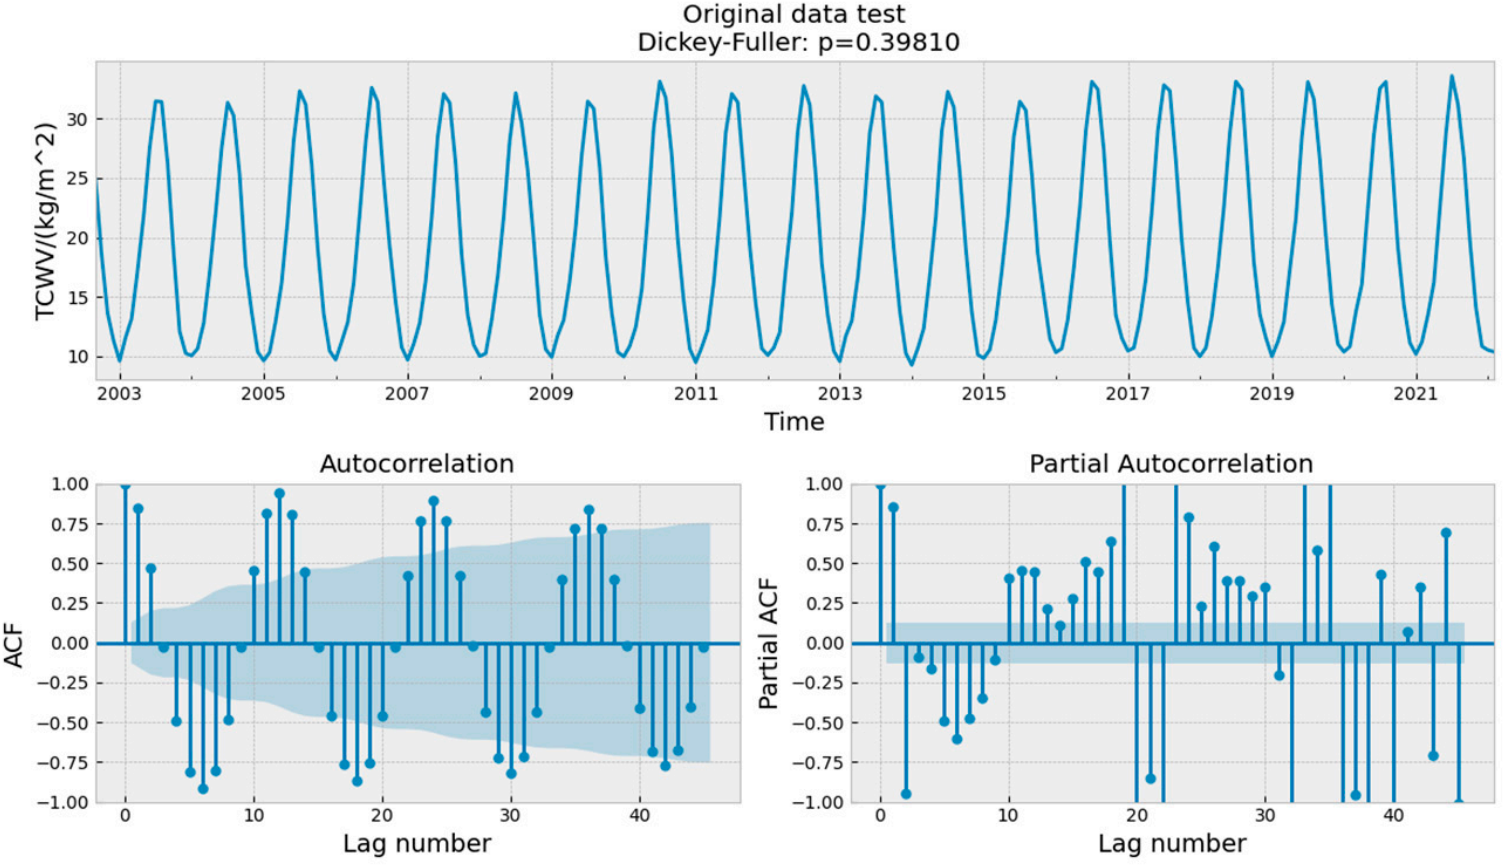
\includegraphics[width=0.8\paperwidth]{static/course_2_img/acf_pacf.PNG}}
  \hspace*{15pt}\hbox{\scriptsize Credit:\thinspace{\scriptsize\itshape Shangguan, S et al. \emph{Atmosphere} (2022)}} 
\end{frame}

\begin{frame}{Example: Autocorrelation of the US CPI }
  
 \makebox[\linewidth]{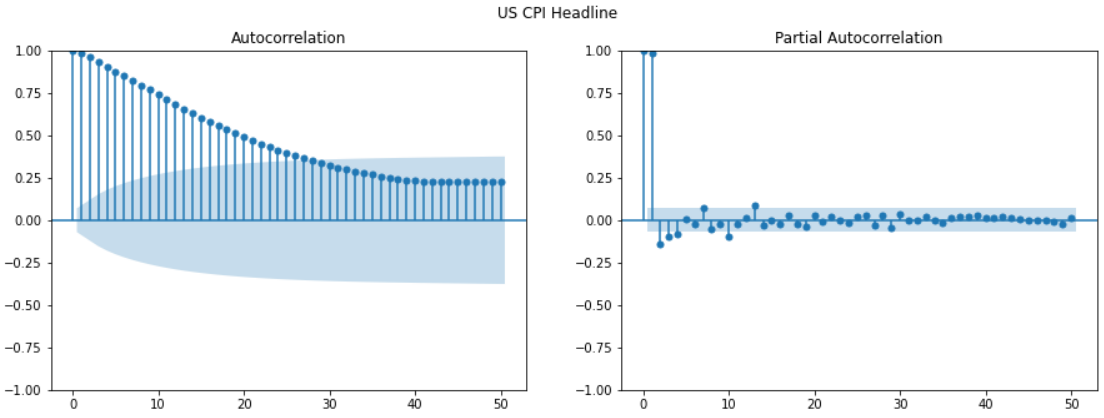
\includegraphics[width=\textwidth]{static/course_2_img/cpi_autocorrelogram.PNG}}
 
 \begin{itemize}
     \item Highly significant autocorrelation in the first 20 lags
     \item However, PACF displays one single significant bar at the first lag
     \item Relation between t and t-s, s >1 goes through t-1
     \item AR(1) model is the best fit to the time series
 \end{itemize}
\end{frame}

\begin{frame}{Example: Autocorrelation of the SP500}
   \begin{exampleblock}{Fact N2:}
    The autocorrelations of assets returns are often insignificant, except for intraday time scales (around 20 minutes) for which the microstructure effects come into play
  \end{exampleblock}
  
 \makebox[\linewidth]{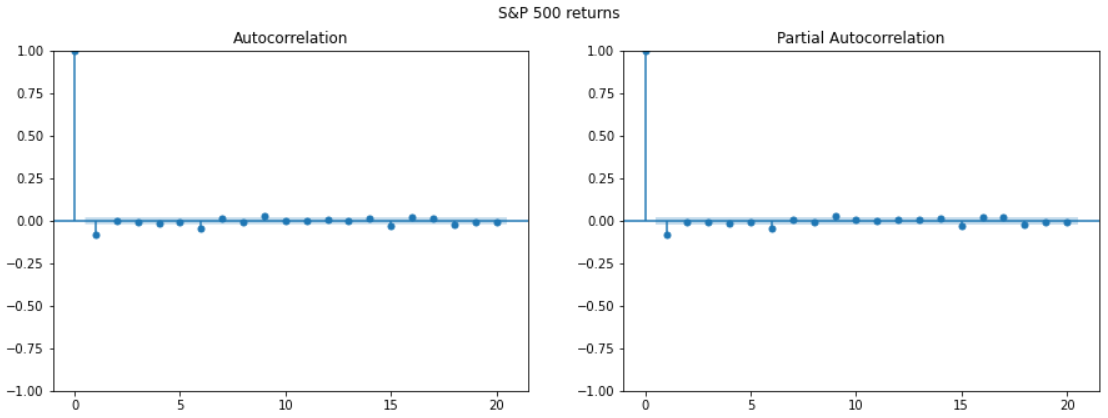
\includegraphics[width=.8\textwidth]{static/course_2_img/SP500_ret.PNG}}

 \begin{itemize}
     \item The fact that returns hardly show any serial correlation does not mean that they are independent
     \item Financial time series are difficult to model. That's why we need Quants!
 \end{itemize}
 
\end{frame}
\subsection{Heavy Tails}
\begin{frame}{Heavy Tails}
  \begin{exampleblock}{Fact N3: Heavy Tails}
    The probability distribution of many financial variables, including asset returns, often exhibit \textbf{heavier tails} than those of a normal distribution
  \end{exampleblock}

  \begin{itemize}
  \item "Heavier tails" are rigorously defined by the kurtosis, which is the fourth-order moment (see before)
  \item Mandelbrot (1963) recognized the heavy-tailed, highly peaked nature of certain financial time series
  \item These heavy tails can be explained by risk aversion, heard behavior, and market microstructure (illiquidity, asymmetric information, etc.)
  \end{itemize}    
\end{frame}


\begin{frame}{Forms of Kurtosis (Fat Tails)}
  There are different shapes of kurtosis:\\ 
 \makebox[\linewidth]{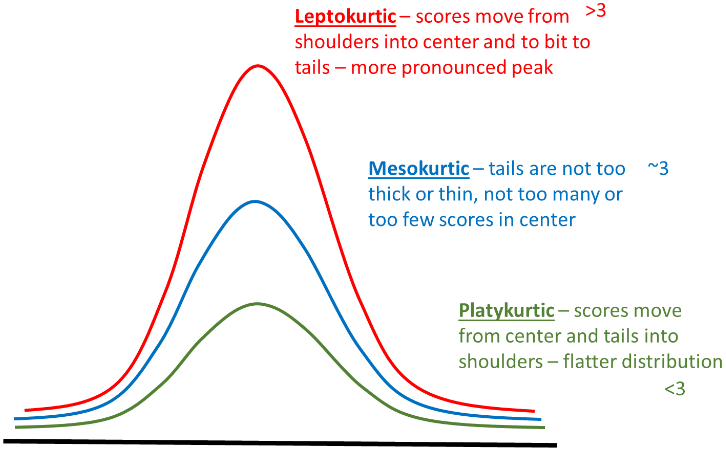
\includegraphics[width=0.8\paperwidth]{static/course_2_img/forms of kurtosis.PNG}}  
\end{frame}
\subsection{Asymmetry}
\begin{frame}{Asymmetry}

  \begin{exampleblock}{Fact N4: Asymmetry}
    The distribution of many financial variables, including asset returns, are often \textbf{asymmetric} and \textbf{negatively skewed}
  \end{exampleblock}

  \begin{itemize}
  \item Asymmetry is defined by the skewness, which is the third-order moment
  \item This reflects the fact that the downturns of financial markets are often much steeper than the recoveries
  \begin{itemize}
    \item Investors tend to react more strongly to negative news than to positive news 
    \item Rush toward the exit door/ flight to safety
  \end{itemize}
  \end{itemize}
\end{frame}


\begin{frame}{Skewness}
  There are different shapes of kurtosis 
  \makebox[\linewidth]{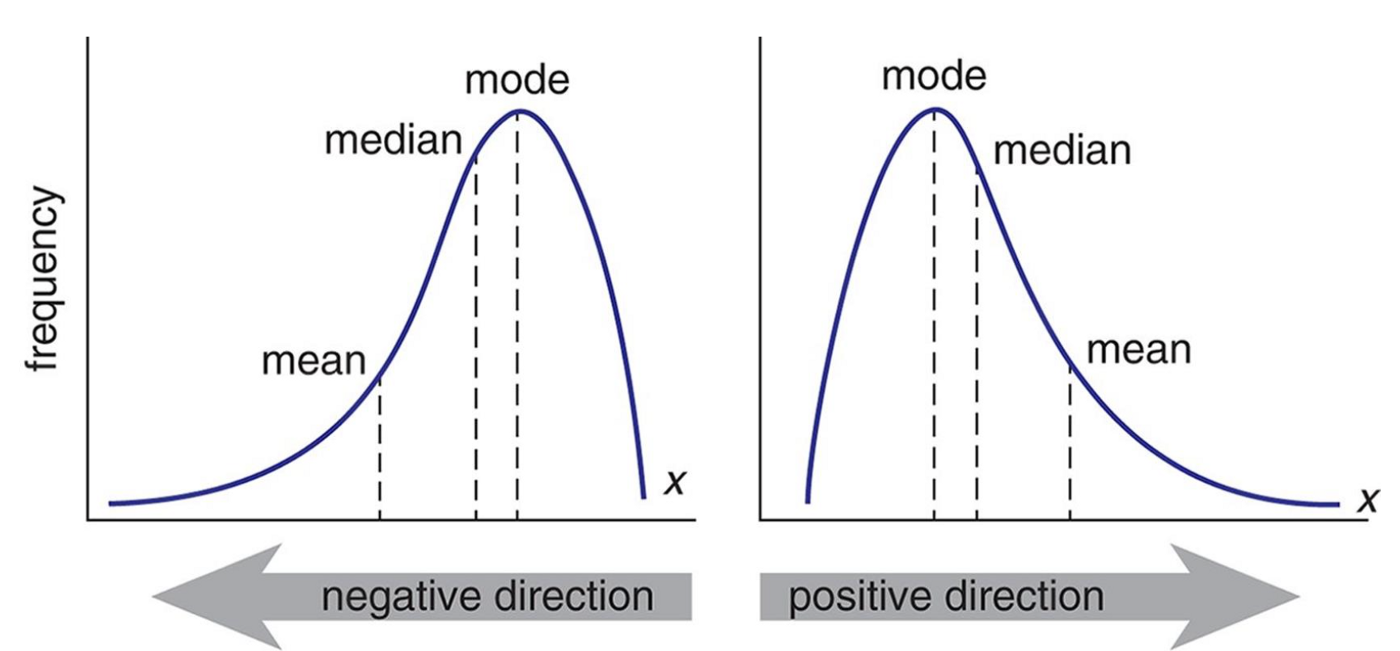
\includegraphics[width=0.8\paperwidth]{static/course_2_img/skewness.PNG}}
  \hspace*{15pt}\hbox{\scriptsize Credit:\thinspace{\scriptsize\itshape Towards Data Science}} 
  \begin{itemize}
      \item Skew $= 0 \Rightarrow$  Symmetric distribution $\Rightarrow$ \textbf{Mean} = \textbf{Median}
      \item Skew $\geq 0 \Rightarrow$ Positive skew implies that the \textbf{Mean} is driven by a small number of high values
      \item Skew $\leq 0 \Rightarrow$ Positive skew implies that the \textbf{Mean} is driven by a small number of small values
  \end{itemize}
  
\end{frame}

\subsection{Volatility Clustering}
\begin{frame}{Volatility Clustering}
  \begin{exampleblock}{Fact N5: Volatility Clustering}
    \begin{itemize}
    \item Large price changes tend to be followed by large price changes (up and down)
    \item It means that returns with large absolute values or large squares occur in clusters    
    \end{itemize}    
  \end{exampleblock}
      \textbf{Note:}\\ volatility clustering is the consequence of the autocorrelation of the squared returns
\end{frame}


\begin{frame}{Volatility Regimes: US VIX}
  Periods of tranquility alternate with periods of high volatility (volatility regimes)\\

  \begin{figure}
      \centering
      \caption{The VIX is the implied volatility of the US SP 500}
      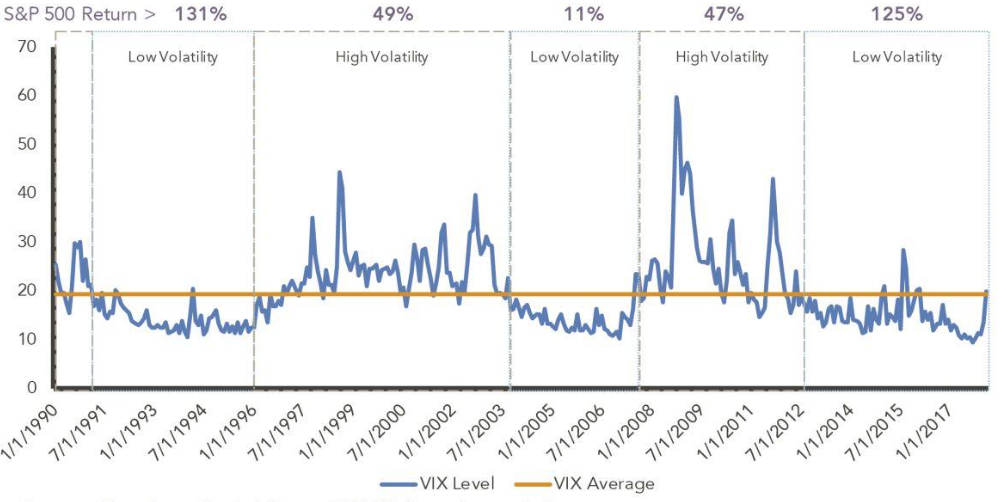
\includegraphics[width=.9\textwidth]{static/course_2_img/vix volatility.PNG}
  \end{figure}
\end{frame}




% \begin{frame}{Aggregational Gaussanity In Practice}
%   \makebox[\linewidth]{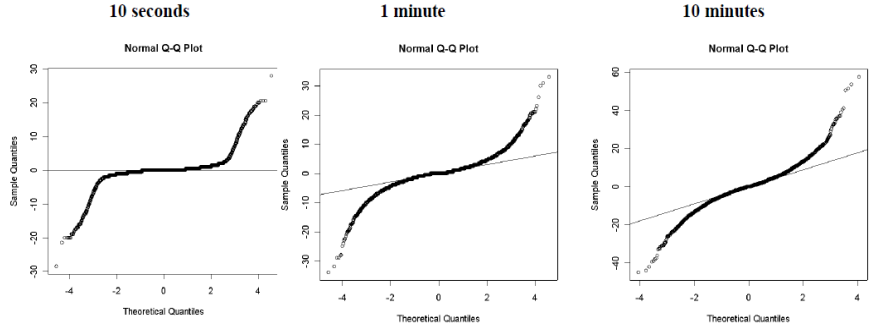
\includegraphics[width=0.8\paperwidth]{static/course_2_img/aggregational gaussianity.PNG}}
%   \hspace*{15pt}\hbox{\scriptsize Credit:\thinspace{\scriptsize\itshape Christophe Hurlin}} 
% \end{frame}

\subsection{Long Range Dependence}
\begin{frame}{Long Range Dependence}
  \begin{exampleblock}{Fact N6: Long Memory}
    At the difference of returns, squared returns and absolute returns exhibit significant autocorrelations (\textbf{long-memory})
  \end{exampleblock}
  {The ARCH effect}
  \begin{itemize}
  \item The autocorrelation of the squared returns is called the \textbf{ARCH effect} (auto-regressive conditional heteroskedasticity)
  \item ARCH effect is important in finance, because it describes patterns in the dynamic of financial volatility 
  \item Those autocorrelations become weaker and less persistent when the sampling interval is increased to a week or a month
  \end{itemize}
  
\end{frame}


\begin{frame}{Long Range Dependence}
  SP 500 Returns (left) and squared returns (right) \\

\medskip
  
 \makebox[\linewidth]{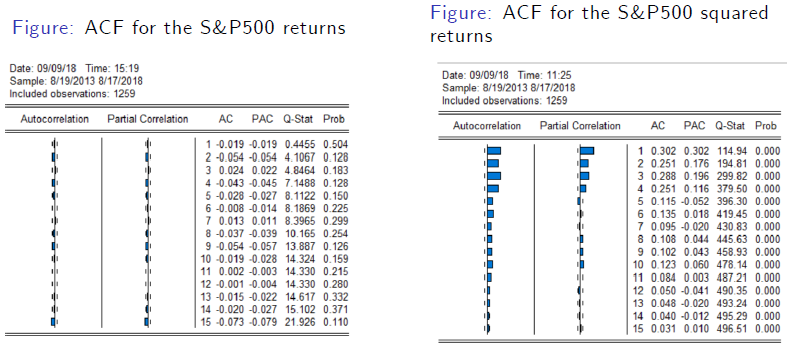
\includegraphics[width=0.8\paperwidth]{static/course_2_img/long range dependence.PNG}}  
\end{frame}

\subsection{Leverage Effect}
\begin{frame}{Leverage Effect}

  \begin{exampleblock}{Fact N7: the Leverage Effect}
Assets returns are negatively correlated with the changes in their volatilities    
  \end{exampleblock}
  \medskip
  Financial explanations
    \begin{itemize}
    \item An asset price declines, companies mechanically become more leveraged (debt-to-equity ratio up) and riskier: therefore, their stock prices become more volatile
    \item On the other hand, when stock prices become more volatile, investors demand high returns, and hence stock prices go down
    \item Volatilities caused by price decline are typically larger than prices appreciation due to declined volatilities
    \end{itemize}
\end{frame}

\subsection{Aggregational Gaussianity}
\begin{frame}{Aggregational Gaussianity}

  \begin{exampleblock}{Fact N8: Aggregational Gaussianity}
    \begin{itemize}
    \item Asset returns over $k$ days is simply the aggregation of $k$ daily returns
    \item When the time horizon $k$ increases, the central limit theory says that the distribution of returns over a long-time horizon (a few months) tends toward a \textbf{normal distribution}
    \end{itemize}
  \end{exampleblock}


  \begin{itemize}
  \item Aggregational gaussianity implies that over long horizons, the peculiarities of financial time series over short-term horizons (skewness, kurtosis, ARCH effect etc.) tend to vanish
  \item However, in finance, people are mostly interested in relatively short-term movements, suggesting that working under the Gaussianity assumption is often not appropriate
  \end{itemize}
  
\end{frame}


\section{Useful Techniques: Differencing}

\begin{frame}{Differencing}
  \begin{wideitemize}
  \item Differencing helps to \textbf{stabilize the mean}
  \item The differenced series is the \emph{change} (or first difference) between each observation in the original series: $y'_t = y_t - y_{t-1}$
  \item The differenced series will have only $T-1$ values since it is not possible to calculate a difference $y'_1$ for the first observation
  \end{wideitemize}

\end{frame}

\begin{frame}{Differencing}
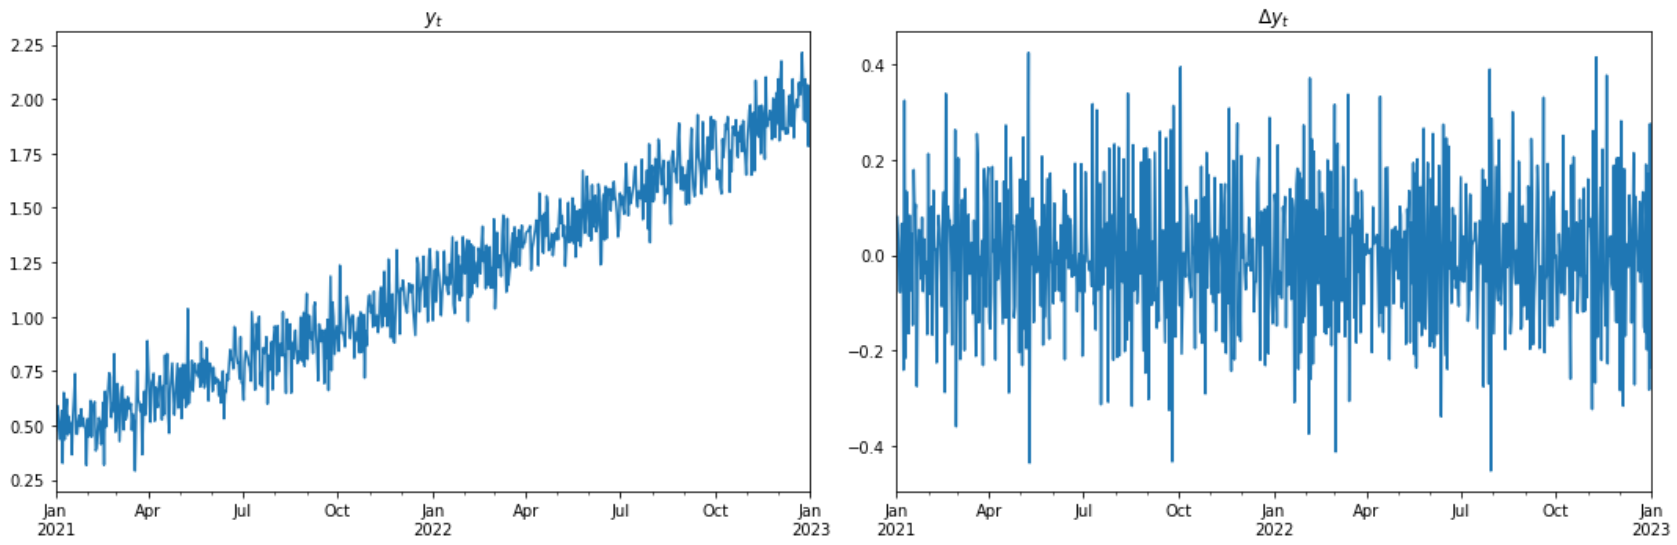
\includegraphics[width=\textwidth]{static/course_2_img/differencing.png}

Suppose $$y_t = \beta_0 + \beta_1 \times t + \epsilon_t$$
Let $$z_t = \Delta y_t = y_t - y_{t-1}$$
\begin{align*}
z_t &= (\beta_0 + \beta_1 \times t+ \epsilon_t) - (\beta_0 + \beta_1 \times (t-1) + \epsilon_{t-1})\\
    &= \beta_1 + (\epsilon_t - \epsilon_{t-1})\\
    &= \beta_1 + \nu_t \sim  N(0, \sqrt{2\sigma^2}) \\
\end{align*}


    
\end{frame}

\begin{frame}{Second-Order Differencing}

  Occasionally, the differenced data will not appear stationary and it may be necessary to differentiate the data a second time:\\

  \medskip
  
  \begin{equation*}
    y''_{t} = y'_t - y'_{t-1} = (y_t - y_{t-1}) - (y_{t-1} - y_{t-2})
  \end{equation*}

  \medskip

  \begin{itemize}
  \item $y''_{t}$ will have $T-2$ values
  \item In practice, it is almost never necessary to go beyond second-order differences
  \end{itemize}
  
\end{frame}


\begin{frame}{Seasonal Differencing}

  \begin{block}{Definition: Seasonal Difference}
    A seasonal difference is a difference between an observation and the corresponding observation from the previous year

    \begin{equation*}
      y'_t = y_t - y_{t-m}
    \end{equation*}

    where $m$ = number of seasons


    \begin{itemize}
    \item For monthly data, $m = 12$
    \item For quarterly data, $m = 4$      
    \end{itemize}
    
  \end{block}
\end{frame}


\begin{frame}{Differencing in Practice}

  When both seasonal and first differences are applied:

  \begin{wideitemize}
    \item It makes no difference which one is done first - the result will be the same
    \item If seasonality is strong, we recommend that seasonal differencing be done first because sometimes the resulting series will be stationary and there will be no need for the further first difference
    \item It is important that, if differencing is used, the differences are \textbf{interpretable}: for instance, taking lag 3 differences for yearly data is difficult to interpret
  \end{wideitemize}
\end{frame}


\section{AR, MA, ARMA, ARIMA, SARIMA models}
\begin{frame}
  \frametitle{Autoregressive (AR) Models}

  \begin{block}{Definition}
    \begin{equation*}
      y_t = c + \phi_1 y_{t-1} + \phi_2 y_{t-2} + \dots + \phi_P y_{t-p} + \epsilon_t
    \end{equation*}

    \begin{itemize}
    \item where $\epsilon_t$ is a white noise
    \item This is a multiple regression with \textbf{lagged variables}
    \end{itemize}    
  \end{block}
\medskip\medskip
  \makebox[\linewidth]{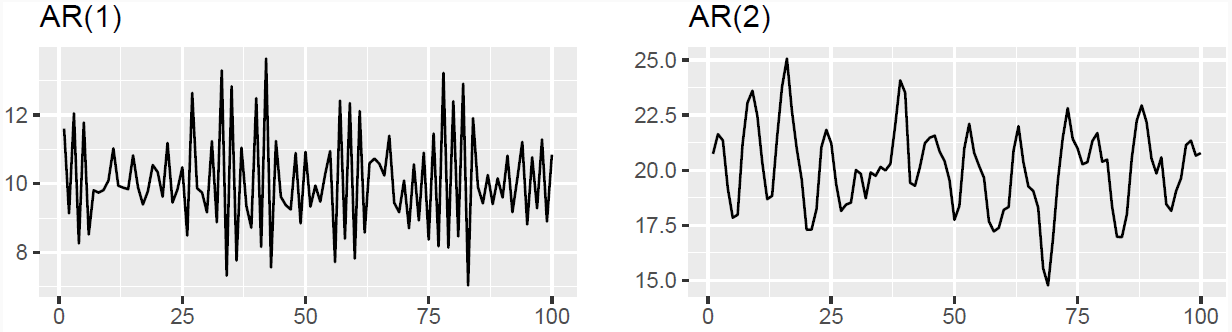
\includegraphics[width=0.7\paperwidth]{static/course_2_img/ar1_ar2.PNG}}   
\end{frame}


\begin{frame}
  \frametitle{AR(1) Model}
  \begin{block}{Specification}
    \begin{equation*}
      y_t = c + \phi_1 y_{t-1} + \epsilon_t
    \end{equation*}
  \end{block}

  \begin{itemize}
  \item When $\phi_1=0$, $y_t$ is equivalent to a \textbf{white noise}
  \item When $\phi_1=1$ and $c=0$, $y_t$ is equivalent to a \textbf{random walk}
  \item When $\phi_1=1$ and $c \neq 0$, $y_t$ is equivalent to a \textbf{random walk with drift}
  \item When $\phi_1<0$ and $c=0$, $y_t$ tends to oscillate between positive and negative values 
  \end{itemize}
  
\end{frame}


\begin{frame}
  \frametitle{Stationarity Conditions}
  To restrict AR models to stationary data, some constraints on the coefficients are needed\\
\medskip
  For low lags orders, the stationarity conditions are simply:\\
  
  \begin{wideitemize}
  \item For $p=1$: $-1 < \phi_1 < 1$
  \item For $p=2$:  $-1 < \phi_2 < 1$, $ \phi_1 + \phi_2 < 1$ and $ \phi_2 - \phi_1 < 1$
  \item More complex conditions hold for $p \geq 3$
  \item Estimation software (R, Python, Eviews, etc.) takes care of this
  \end{wideitemize}
  
\end{frame}

\begin{frame}{How to identify the order of an AR process}
    By definition, PACF gives the direct effect of lag k on the current value of the time series
    $$y_t =\alpha -0.5 \times y_{t-1} + 0.8 \times y_{t-2} + 0.4 \times y_{t-3} + \epsilon_t$$
    \vspace{2pt}
    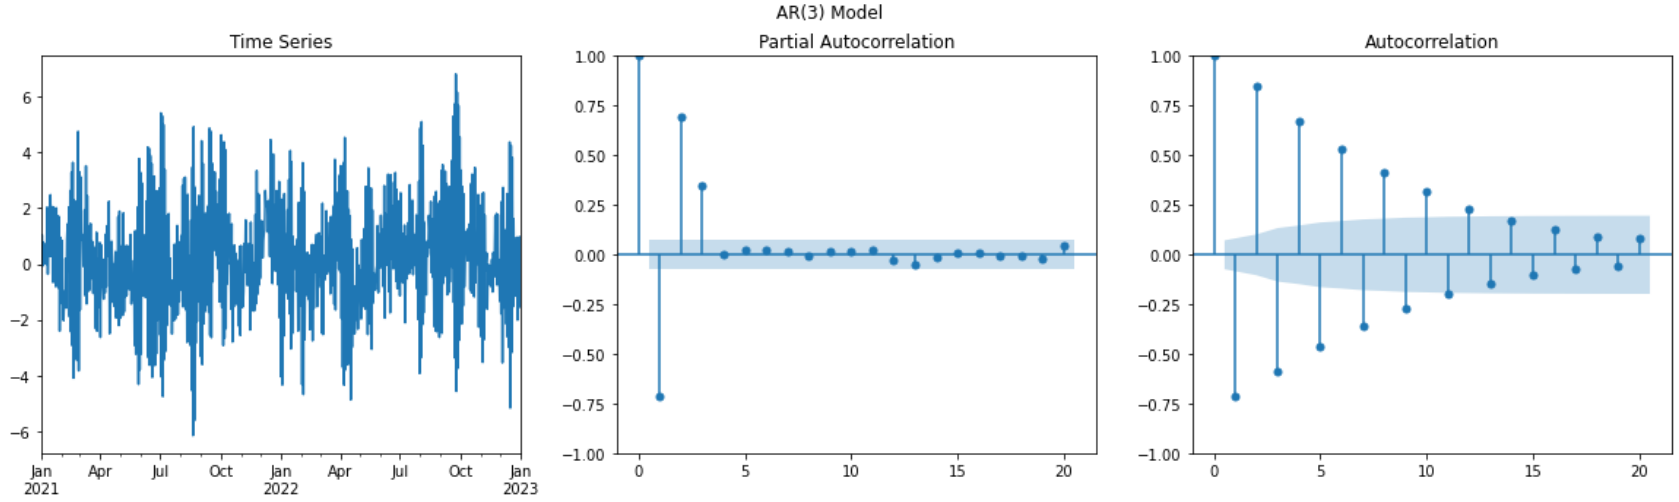
\includegraphics[width=\textwidth] {static/course_2_img/AR_PACF.png}
\end{frame}


\begin{frame}{MA: Moving Average Model}
  \begin{block}{Definition: Moving Average Model}
    \begin{equation*}
      y_t = c + \epsilon_t + \theta_1 \epsilon_{t-1} + \theta_2 \epsilon_{t-2} + \dots + \theta_q \epsilon_{t-q}
    \end{equation*}
    \begin{itemize}
    \item $\epsilon_t$ is a white noise
    \item This is a multiple regression with \textbf{past errors} as predictors
    \item Do NOT confuse this with \emph{moving average smoothing}!
    \end{itemize}    
  \end{block}

  \makebox[\linewidth]{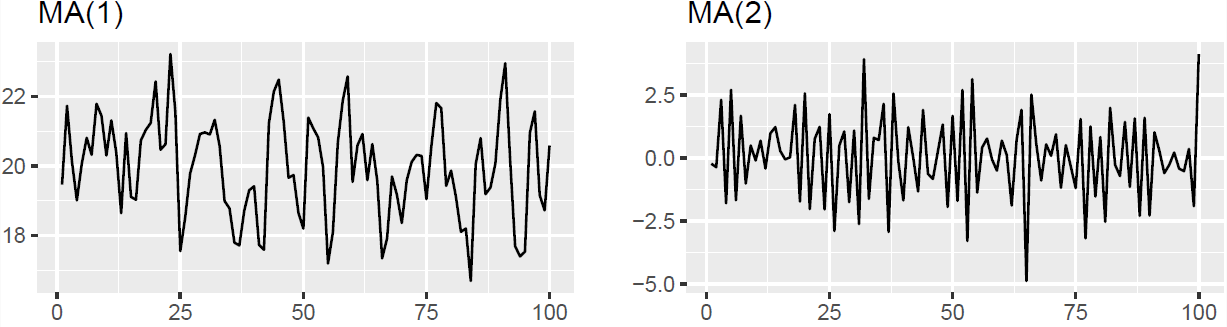
\includegraphics[width=0.7\paperwidth]{static/course_2_img/ma1_ma2.PNG}}     
\end{frame}

\begin{frame}{How to identify the order of an MA process}
Suppose the following MA(q) model
$$MA(q):\quad X_t = \mu +\phi_1\epsilon_{t-1}+\phi_2\epsilon_{t-2}+...+\phi_q\epsilon_{t-q}+\epsilon_{t}$$
The ACF computes the correlation between $X_t$ and $X_{t-k}$
$$ \mathbb{C}orr(X-t, X_{t-k}) = E[X_tX_{t-k}] - E[X_t]E[X_{t-k}]$$
\begin{align*}
X_t &:[\epsilon_t, \epsilon_{t-1}, \epsilon_{t-2}, ..., \epsilon_{t-q}] \\
X_{t-k}&:[\epsilon_{t-k}, \epsilon_{t-k-1}, \epsilon_{t-k-2}, ..., \epsilon_{t-k-q}]
\end{align*}

\begin{align*}
\mathbb{C}orr(X-t, X_{t-k}) & \neq 0 \quad IF  \quad t-q \leq t-k \Rightarrow k \leq q \\
                   & = 0 \quad otherwise
\end{align*}

From an ACF we can deduce the order of the MA model as the lag on which the correlation turns to 0
\end{frame}

\begin{frame}{Example}
$$MA(3):\quad X_t = 50 +5\times\epsilon_{t-1}+3\times\epsilon_{t-2}+ 10\times\epsilon_{t-3}+\epsilon_{t}$$
\vspace{2pt}
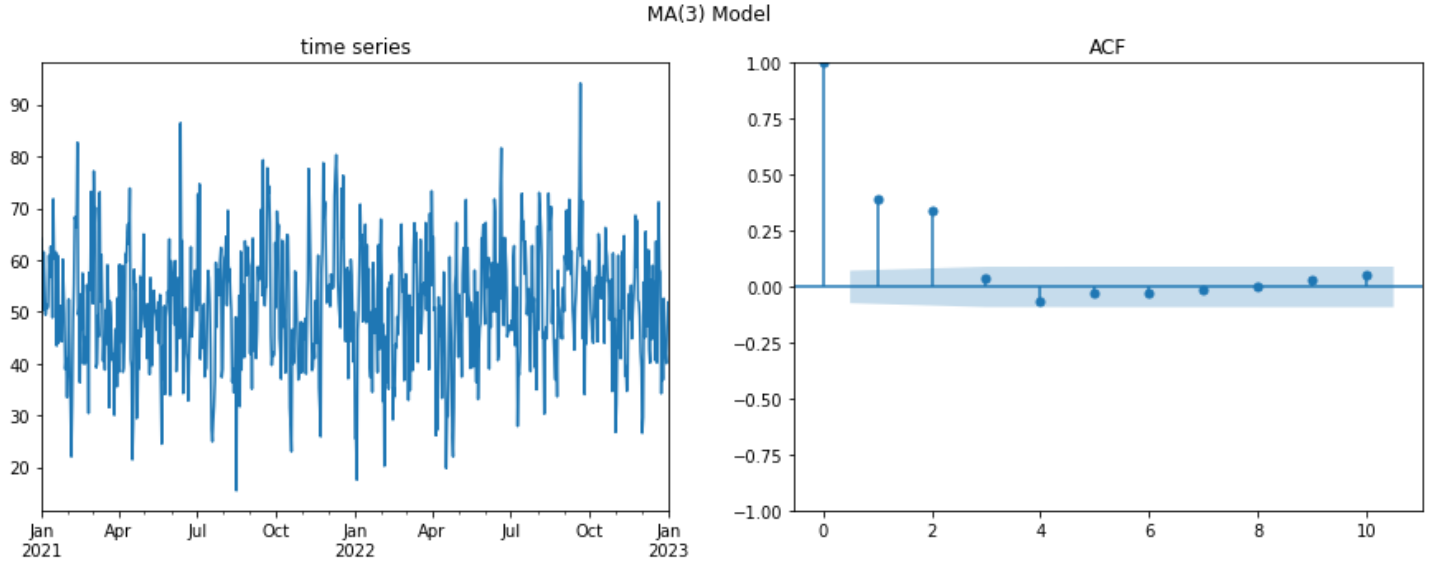
\includegraphics[width=\textwidth]{static/course_2_img/MA_ACF.png}
    
\end{frame}


\begin{frame}
  \frametitle{Wold Decomposition: From AR(p) to MA($\infty$) Model}

  \begin{block}{Wold Decomposition}
    It is possible to write any \textbf{stationary} AR(p) model as an MA($\infty$)
  \end{block}

  \begin{itemize}
  \item Intuitive: just go backward!
  \item $y_t = \phi_1 \underbrace{y_{t-1}}_{} + \epsilon_t$
  \item $y_t = \phi_1 (\phi_1 y_{t-1} + \epsilon_{t-1}) + \epsilon_t$ = $\phi_1^2 y_{t-2} + \phi_1\epsilon_{t-1} + \epsilon_t$
  \item $\dots$
  \item Providing that $1 < \ \phi_1 \ < 1$:
    \begin{align*}
      y_t &= \epsilon_t + \phi_1 \epsilon_{t-1} + \phi_1^2 \epsilon_{t-2} + \phi_1^3 \epsilon_{t-3} + \dots\\
      &= \epsilon_t + \sum_{i=1}^{\infty} { \phi_i \epsilon_{t-i}} 
    \end{align*}
  \end{itemize}  
\end{frame}


\begin{frame}
  \frametitle{Invertibility: From MA(q) to AR($\infty$)}

  \begin{wideitemize}
    \item Under certain conditions, an MA(1) process can be written as an AR($\infty$) process
    \item In this case, the MA model is said to be \textbf{invertible}
    \item Invertible models have some mathematical properties that make them easier to use in practice
    \item This is intuitive: AR processes are embedding new information on the most recent lags 

  \end{wideitemize}
  
\end{frame}


\begin{frame}
  \frametitle{ARMA(p, q) Model}
  \begin{block}{Specification}
    \begin{equation*}
      y_t = c + \underbrace{\phi_1 y_{t-1} + \dots + \phi_p y_{t-p}}_{\text{AR}} + \underbrace{\theta_1 \epsilon_{t-1} + \dots + \theta_q \epsilon_{t-q}}_{\text{MA}} + \epsilon_t
    \end{equation*}
  \end{block}

  \medskip

  \begin{itemize}
  \item The predictors include both \textbf{lagged values of $y_t$} and \textbf{lagged errors}
  \item Important specification: the future value of the series depends both on the past values it took (dynamic), as well as recent random noise/error term 
  \item This simple model is "learning" both from the dynamic of the past values and from its inherent randomness
  \item Conditions on AR coefficients ensure \textbf{stationarity}
  \item Conditions on MA coefficients ensure \textbf{invertibility}
  \end{itemize}
  
\end{frame}

\begin{frame}
  \frametitle{Autoregressive Integrated Moving Average (ARIMA)}

  ARIMA: AR\textbf{I}MA stands for: Autoregressive \textbf{Integrated} Moving Average model

  \begin{itemize}
  \item Basically, it is a non-stationary model that can be made stationary by differencing
  \item $(1-B)^d y_t$ follows an ARMA model: $d$ is the degree of differencing
  \item Once differenced $d$ times, it is stationary and behaves as an ARMA model
  \end{itemize}  
\end{frame}


\begin{frame}
  \frametitle{Generalization}

  \begin{wideitemize}
  \item $ARIMA(p, d, q)$ where $p$ is the autoregressive order, $d$ the degree of differencing and $q$ the order of the moving average part
  \item All linear models we discussed are special cases of the ARIMA model:
    \begin{wideitemize}
    \item White noise model: $ARIMA(0, 0, 0)$
    \item Random walk: $ARIMA(0, 1, 0)$ with no constant
    \item Random walk with drift: $ARIMA(0, 1, 0)$ with constant  
    \item $AR(p) = ARIMA(p, 0, 0)$ , $MA(q) = ARIMA(0, 0, q)$
    \end{wideitemize}
  \end{wideitemize}
    
\end{frame}

\begin{frame}
  \frametitle{Seasonal ARIMA (SARIMA)}

  \begin{block}{Specification}
    ARIMA  $ \underbrace{(p, d, q)}_{_{\text{Non-Seasonal part of the model}}} \qquad \qquad \underbrace{(P, D, Q)_m}_{\text{Seasonal part of the model}}$\\
    where $m$ is the number of observations in a cycle
  \end{block}

\medskip
\pause
    
Example: $ARIMA(1,1,1)(1,1,1)_4$, without constant

\begin{equation*}
  \underbrace{(1-\phi_1B)}_{\text{Non-Seas. AR1}} \underbrace{(1-\Phi_1B^4)}_{\text{Seas. AR1}}\underbrace{(1-B)}_{\text{Non-Seas. Diff.}} \quad = \quad \underbrace{(1+\theta_1 B)}_{\text{Non-seas. MA(1)}} \underbrace{(1+\Theta_1 B^4)}_{\text{Seasonal MA(1)}}\underbrace{(1-B^4)}_{\text{Seas. Diff.}}\epsilon_t
\end{equation*}

\medskip

  All factors can be multiplied to obtain the model's component form
\end{frame}



\begin{frame}
  \frametitle{Intuition}

  The seasonal part of an AR or MA model will be seen in the seasonal lags of the PACF and ACF


  \begin{exampleblock}{$ARIMA(0,0,0)(0,0,1)_{12}$  will show}

    \begin{itemize}
    \item A spike at lag 12 in the ACF but no other significant spikes
    \item The PACF will show exponential decay in the seasonal lags; that is, at lags 12, 24, 36, etc.
    \end{itemize}
    
  \end{exampleblock}
  
\medskip

  \begin{exampleblock}{$ARIMA(0,0,0)(1,0,0)_{12}$  will show}

    \begin{itemize}
    \item Exponential lags in the seasonal lags of the ACF
    \item A single significant spike at lag 12 in the PACF
    \end{itemize}
    
  \end{exampleblock}

\end{frame}


\begin{frame}
  \frametitle{Treatment of Seasonality}

  \begin{wideitemize}
    \item Daily data can exhibit multiple seasonal periodicities. This is a complication for all high-frequency forecasting problems: day in the month, day in the week, etc.
    \item This comes with additional complexity:
      \begin{itemize}
        \item Months has different number of days
        \item Leap years with different number of days
        \item Weeks do not align with daily cycles (the year is not divisible in an exact number of weeks)
        \end{itemize}
      \item Seasonality can be irregular: Ramadan and some other religious festivities for instance
      \item We use two approaches to deal with complex seasonality
        \begin{enumerate}
        \item Trigonometric representation of seasonality
        \item Simplification of seasonal terms
        \end{enumerate}
  \end{wideitemize}
  
\end{frame}


\begin{frame}
  \frametitle{Problems of an ARIMA with Many Binary Variables}

  \begin{wideitemize}
  \item Often, central banks forecast currency in circulation by including a large number of binary variables (“dummies”) to capture different seasonality patterns. This is called \textbf{binary seasonality}

  \item In general, this approach should be discouraged, because:
    \begin{itemize}
    \item Including a large number of variables imply to estimate many more parameters, hence \textbf{adding parametric noise to the model}
    \item Many parameters are not relevant/useful, \textbf{increasing noise/signal ratio}
    \item Reducing the degrees of freedom spurs the \textbf{risk of overfit}
    \end{itemize}
    
  \item We tested a large number of models in different countries, confirming the relatively bad performance of ARIMA with binary seasonality
    
  \end{wideitemize}

\end{frame}


\section{Empirical Strategy}

\begin{frame}
  \frametitle{Empirical Strategy}
  The general approach of (financial) econometrics is as follows:\\
  \smallskip

  \begin{wideenumerate}
  \item Specification of the model
  \item Estimation of the parameters
  \item Diagnostic tests
    \begin{itemize}
    \item Significance tests
    \item Specification tests
    \item Backtesting tests
    \item etc.
    \end{itemize}
  \item Interpretation and use of the model (forecasting, historical studies, etc.)
  \end{wideenumerate}
\end{frame}

\begin{frame}
  \frametitle{How to Specify an Appropriate Time Series Model}
  \begin{wideenumerate}
    \item Study some \textbf{statistical properties} of the observed data $\{x_t\}$, for instance, the \textbf{stationarity}, the patterns of the autocorrelation function \textbf{ACF}, or the \textbf{partial autocorrelation function}, etc.
    \item Compare these properties to the theoretical properties of some \textbf{typical time series models}, such as AR, MA, ARIMA, SARIMA, etc.
    \item Choose the most appropriate model and \textbf{estimate its parameters}
    \item Use this model for forecasting
  \end{wideenumerate}
\end{frame}

\begin{frame} % Need to be redone
  \frametitle{Modeling Process}
  \makebox[\linewidth]{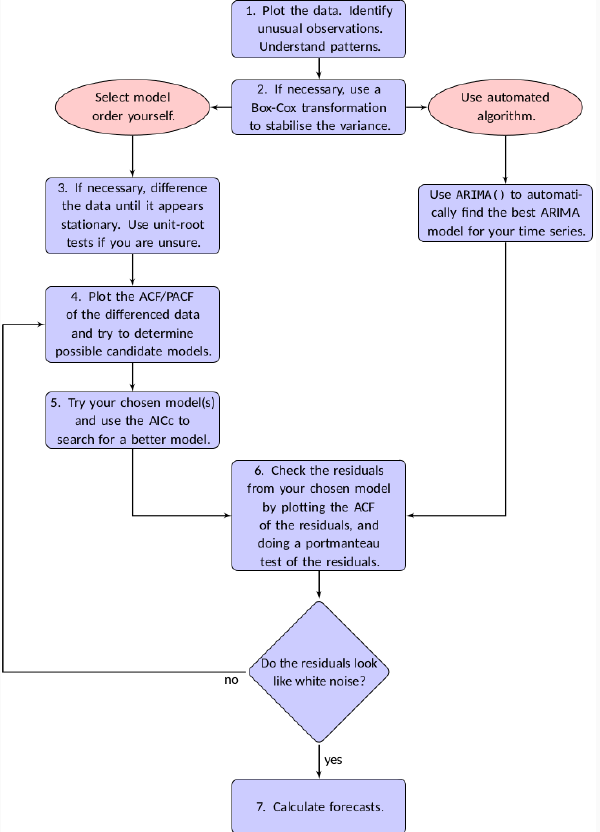
\includegraphics[height=.85\paperheight]{static/course_2_img/model_process.PNG}}     
\end{frame}


\begin{frame}
  \frametitle{General Approach}
  \begin{itemize}
  \item \textbf{Plot the data}. Identify any unusual observations
  \item If necessary, \textbf{transform the data} (using a Box-Cox transformation) to stabilize the variance
  \item If the data are non-stationary, \textbf{first-difference} it until stationarity
  \item \textbf{Examine the ACF/PACF}: is an $AR(p)$ or $MA(q)$ reasonable assumptions
  \item Try your chosen models: use AIC to compare with other models
  \item Plot the residuals, look at the residuals ACF. Residuals should look like a \textbf{white noise}. As long as the residuals of the model have structure, the model is not capturing the whole signal but only part of it
  \item Once the residuals look like a white noise, \textbf{compute the forecasts}    
  \end{itemize}
\end{frame}

\begin{frame}
    \centering
    \Huge Thank you for you attention !
\end{frame}


\appendix
\begin{frame}{Intuitive Interpretation}
   Weak stationarity means that the stochastic process oscillates around a constant level, is not trending, and has the following properties:\\
  
  \begin{wideenumerate}
  \item The mean and time-covariance are constant over time

\item Because the time-covariance is constant over time, it implies that the variance is also constant over time
  \begin{equation*}
\mathbb{V}(X_t) = \mathbb{C}ov(X_t, X_{t}) = \gamma(0) \qquad \forall \ t \ \in \ \mathbb{Z}
  \end{equation*}
\item $\mathbb{C}ov(X_t, X_{t}) = \gamma(h) \qquad \forall \ h \ \in \ \mathbb{Z}$ can be interpreted as "\emph{covariance doesn't change when shifted in time}"
  \begin{equation*}
\mathbb{C}ov(X_r, X_s) = \mathbb{C}ov(X_{r+t}, X_{s+t}) \qquad \forall \ (r, s, t) \ \in \ \mathbb{Z}^3
  \end{equation*}
  
  \end{wideenumerate}
\end{frame}
% Add charts
\begin{frame}{Backshift Notation}

  \begin{block}{Notation}
    The backshift notational device, $B$ is used as follows:\\

    \begin{equation*}
      B y_t = y_{t-1}
    \end{equation*}
  \end{block}

    
    \begin{itemize}
    \item   $B$ operating on $y_t$ has the effect of \textbf{shifting the data back one period}
    \item   Two applications of $B$ to $y_t$ shifts the data back \textbf{two periods}
      \begin{equation*}
        B(By_t) = B^2 y_t = y_{t-2}
      \end{equation*}
    \end{itemize}
    
$B$ depends on the period/frequency considered. Shifting monthly data by a year supposes using $B^{12}$

\end{frame}


\begin{frame}{Relationship with Differencing}
  Importantly, the backshift operator is convenient for describing differencing\\

  \medskip
  
  \begin{exampleblock}{Backshift Operator and Differencing}
    $$y'_t = y_t - y_{t-1} = y_t - By_t = (1-B)y_t$$
  \end{exampleblock}


  \begin{itemize}
    \item Likewise, second-order differences are obtained with $y''_t = (1-B)^2y_t$  
    \item Pay attention !! The second-order difference is not second difference 
      \begin{itemize}
      \item Second order difference: $(1-B)^2 y_t = y''_t = (y_t - y_{t-1}) - (y_{t-1} - y_{t-2})$
      \item Second difference: $1-B^2 y_t = y_t - y_{t-2}$
      \end{itemize}
  \end{itemize}
  
\end{frame}
\begin{frame}
  \frametitle{Stationarity Conditions}
  To restrict AR models to stationary data, some constraints on the coefficients are needed

  \begin{alertblock}{General Condition for Stationarity}
    Complex roots of the polynomial $\mathcal{P}(z) = 1 - \phi_1z - \phi_2 z^{2} - \dots \phi_p z^{p}$ lie outside the unit circle of the complex plane
  \end{alertblock}

  \begin{wideitemize}
  \item Intuition: For an AR(1) model, the backshift polynomial is $y_t = \phi_1 y_{t-1} + \epsilon_t \ \leftrightarrow \ y_t(1-\phi_1B) = \epsilon_t$
  \item $(1-\phi_1B) = 0 \ \leftrightarrow \ B= \underbrace{\frac{1}{\phi_1}}_{\text{Not explosive}}$
  \item To get the AR expression not explosive, we need $|\frac{1}{\phi_1}| < 1$ and therefore $|\phi_1| > 1$ 
  \end{wideitemize}


  \end{frame}
\begin{frame}
  \frametitle{Invertibility}

  \begin{alertblock}{General Condition for MA(q) Invertibility}
    Complex roots of $1 + \theta_1z + \theta_2 z^2 + \dots + \theta_q z^q$ lie outside the unit circle of the complex plane
  \end{alertblock}

  \smallskip

  \begin{itemize}
  \item For q =1: $-1 \ < \theta_1 \ <1$
  \item For q=2:
    \begin{itemize}
    \item $-1 \ < \theta_2 \ <1$
    \item $\theta_1 + \theta_2 > -1$ and $\theta_1 - \theta_2 \ < 1$
    \end{itemize}
  \item More complicated solutions hold for $q \geq 3$
  \item Estimation software takes care of this
  \end{itemize}
  
\end{frame}

\begin{frame}{What is a White noise ?}
\begin{block}{Definition}
A time series is a white noise if the variables are independent and identically distributed with a mean of zero.
\begin{center}
${\left\{\begin{matrix}
 \forall t, & \Esp[\epsilon_t] = 0 \\
 \forall t, & \Var[\epsilon_t] = \sigma^2 \\
 \forall t,s & (\epsilon_t, \epsilon_{s}) \quad independent \\    
\end{matrix}\right.\}}$    
\end{center}
\end{block}

Why does it matter?
$$y_t = Signal + Noise $$
    \begin{itemize}
        \item Noise is the unpredictable part of the time series that can not be modeled. Complete randomness 
        \item As long as the residuals of the model have structure, the model is not capturing the whole signal but only part of it
        \item Stop modeling when the series of errors from a time series forecast model is behaving like a white noise
    \end{itemize} 
\end{frame}

% \begin{frame}{Statistical Tesk: Dickey-Fuller Test}
% \small
% Dickey-Fuller test is designed to test if a time series following an AR(1) model is stationary
% $$AR(1): \quad y_t =\alpha + \phi_1 \times y_{t-1} + \epsilon_t$$
% Hypothesis testing

% \left\{\begin{matrix}
% H0: & $y_t$ has a unit root   &$\Rightarrow \phi_1 =1$\\
% H1: & $y_t$ has no unit roots &$\Rightarrow \phi_1 < 1$\\ 
% \end{matrix}\right\}.

% $$\Delta y_t =\alpha + \delta \times y_{t-1} + \epsilon_t, \quad where \quad \delta = \phi_1 - 1$$

% Hypothesis testing

% \left\{\begin{matrix}
% H0: & $y_t$ has a unit root  &$\Rightarrow \delta =0$\\
% H1: & $y_t$ has no unit roots  &$\Rightarrow \delta < 0$\\ 
% \end{matrix}\right\}.

% \begin{itemize}
%     \item If the null hypothesis H0 is true $\delta =0$ and $\Delta y_t$ is a  random walk
%     \item compute the t-statistic as per the hypothesis testing of parameter significance,   $w = t_{\hat{\delta}} = \frac{\hat{\delta}}{std(\hat{\delta})}$
%     \item because $y_t$ is not stationary under the null hypothesis, not compared with the t-distribution but with the Dickey-Fuller distribution 
% \end{itemize}
% \end{frame}

\begin{frame}
  \frametitle{Parameters Selection: Algorithm}
  \begin{block}{ARIMA Specification}
    \begin{equation*}
    \phi(B) (1-B)^d y_t = c + \theta(B) \epsilon_t      
    \end{equation*}

    \begin{wideitemize}
      \item Need to select the appropriate order for $p, q, d$
    \end{wideitemize}
    
  \end{block}

\medskip
  
\textbf{Hyndman and Khandasar (2008) selection algorithm}:\\

\begin{wideitemize}
  \item Select the differencing order (=number of differences) \textbf{$d$} and \textbf{$D$} using KPSS test
  \item Select $p, q$ by minimizing AICs
  \item Use stepwise search to traverse model space (= test different combinations of $p, q$ for robustness)
\end{wideitemize}

\end{frame}


\begin{frame}
  \frametitle{Selection Algorithm}
  \begin{alertblock}{Aikaike Information Criteria (AIC)}
    \begin{equation*}
      AIC = -2 \text{log}(L) + 2(p+q+k+1) \left[ 1 + \frac{(p+q+k+2)}{T-p-q-k-2} \right]
    \end{equation*}
    \begin{itemize}
    \item where $L$ is the maximized likelihood fitted to the \emph{differenced data}
    \item and $k$ Degrees of freedom: if the model embeds a constant $c$, $k=1$, else $k=0$
    \end{itemize}    
  \end{alertblock}

  Steps:\\

  \begin{wideenumerate}
  \item Select the current model, with the smallest AIC from the most parsimonious
    \begin{itemize}
    \item ARIMA(0,d, 0), ARIMA(1, d, 0), ARIMA(0, d, 1), ARIMA(1, d, 1) and ARIMA(2, d, 2)
    \end{itemize}
  \item Consider \textbf{variations} of the current model:
    \begin{itemize}
    \item Vary one of $p, q$ from current model by $\pm 1$
    \item $p, q$ both vary from current model by $\pm 1$
    \item Include/exclude the constant $c$ from the current model
    \end{itemize}
  \item The model with the lowest $AIC$ becomes the current model. Repeat step 2 until no lowest AIC can be found (traverse model space)
  \end{wideenumerate}

\end{frame}
\end{document}
